\chapter{Компьютерные науки}

\AddToShipoutPictureBG*{%
  \AtPageUpperLeft{%
    \hspace{\paperwidth}%
    \raisebox{-\baselineskip}{%
      \makebox[-10pt][r]{\textbf{ПМИ}, ИВТ, БИ}
}}}%

\begin{multicols}{2}
    \raggedcolumns
    \section{Регулярные выражения. Теорема Клини об эквивалентности регулярных выражений и
    конечных автоматов.}
    \begin{definition}{}{}
      $\textbf{\text{Алфавит}} \sum$ - любое $\underline{\text{конечное}}$ множество.
  \end{definition}
  
  \begin{definition}{}{}
      $\textbf{\text{Слово}}$  - $\underline{\text{конечная}}$ последовательность символов из алфавита.
  \end{definition}
  
  \begin{definition}{}{}
      $\textbf{\text{Конкатенация}}$  - операция сцепки. Пусть $w, v$ - слова, где $w = aba$, а $v = bb$, тогда конкатенация этих слов: $w \circ v = ababb$
  \end{definition}
  
  \begin{definition}{}{}
      $ \sum^{*}$ - $\text{множество всех слов } \text{над алфавитом } \sum$
  \end{definition}
  
  \begin{definition}{}{}
      $\textbf{Язык } L$ - подмножество множества всех слов $\sum^{*}$.
  \end{definition}
  
  \begin{definition}{}{}
      Пусть $u = ababb$, тогда $u[i]$ - это $\textbf{i-тая буква}$ в слове $u$. $u[1] = a$, $u[i, j] = u[i]\circ u[i + + 1] \circ \dotsc \circ u[j]$, например $u[1,4] = abab$
  \end{definition}
  
  \begin{definition}{}{}
      \textbf{Длина слова } $|w|$ - количество символов в слове $w$.
  \end{definition}
  
  \begin{definition}{}{}
      $\textbf{Пустое слово } \varepsilon$ - специальное слово, для которого выполняется:
      \begin{enumerate}
          \item $\forall w \in \sum^{*} \implies w \circ \varepsilon = \varepsilon \circ w = w$
          \item $|\varepsilon| = 0$
      \end{enumerate}
  \end{definition}
  
  \begin{definition}{}{}
      Пусть $x \in \sum^{*}$, тогда $x^n = \underbrace{x \circ x  \circ \dots \circ x}_{n}$, нулевая степень: $x^0 = \varepsilon$
  
  \end{definition}
  \begin{definition}{}{}
      Слово $u$ называется \textbf{подсловом} слова $w$, если существуют такие слова $x$ и $z$, что $w = x\circ u \circ z$
  \end{definition}
  
  
  \begin{definition}{}{}
      Пусть $w, u \in \sum^{*}$, тогда $|w|_{u}$ - \textbf{количество различных вхождений} слова $u$ в слово $w$ как подслова
  \end{definition}
  Например, пусть $w = ababa$, а $u = aba$, тогда $|w|_u = |w|_{aba} = 2$
  
  \begin{center}
      \textit{Операции на языках}
  \end{center}
  
  \begin{enumerate}
      \item \textbf{Конкатенация}: $X \circ Y = \{ x \circ y | x \in X, y \in Y\}$
      \item \textbf{Возведение в степень:} $X^n = \underbrace{X\circ X \circ \dots \circ X}_{n}$, при $n \geqslant 1$, если же $n = 0$ и $X \neq \varnothing$, то $X^0 = \varepsilon$. Пустое множество возводить в нулевую степень \textbf{нельзя}.
      \item \textbf{Объединение:} $X|Y = X + Y = X \cup Y$
      \item \textbf{Итерация} или \textbf{звёздочка Клини}: $X^{*} = \varepsilon + X + X^2 + X^3 + \dotsc + X^n + \dotsc$
      \item $X^+ = X \circ X^*$
  \end{enumerate}
  P.S. Язык состоящий из одного слова отождествляется со словом, ровно как и слово состоящие из одного символа является буквой алфавита.
  
  \begin{definition}{}{}
      \textbf{Класс регулярных языков REG}:
  \end{definition}
  \begin{enumerate}
      \item $\varnothing \in REG$
      \item $\forall\sigma \in \sum \implies \{\sigma\} \in  REG$
      \item $\forall X, Y \in REG: X \circ Y, X|Y, X^* \in REG$
  \end{enumerate}
  
  Регулярные языки и только они могут быть заданы при помощи регулярных выражений, например выражение $a(a|bb)$ задаёт регулярный язык $L = \{aa, abb\}$.
  \subsection*{Конечные автоматы}
  \begin{definition}{}{}
    \textbf{\text{Конечный автомат }} $\mathcal{A}$ --- устройство, описываемое набором \\$\langle Q$, $\Sigma$, $q_0$, $\delta$, $F \rangle$:
    \begin{enumerate}
        \item {\bfseries\itshape{Q}} - конечное множество состояний автомата;
        \item $\boldsymbol{\Sigma}$ - алфавит, слова над которым обрабатывает автомат;
        \item $\boldsymbol{q_0}$ - начальное состояние автомата;
        \item $\boldsymbol{\delta}$ : $Q \times (\Sigma\cup\{\varepsilon\} ) \rightarrow 2^{Q}$ - функция переходов
        \item $\boldsymbol{F} \subset \boldsymbol{Q}$ - множество принимающих состояний.
    \end{enumerate}
\end{definition}

Напомним, что $2^Q$ - множество всех подмножеств Q (булеан). Запись $f: A \rightarrow B $ означает, что функция определена на всех элементах множества $A$. Мы считаем, что если $\delta (q,\sigma) = \emptyset$, то переход из состояния $q$  по символу $\sigma \in \Sigma \cup \{ \varepsilon \}$ не  определен.


\textbf{Пример 1. Диаграмма Мура}
\begin{center}
    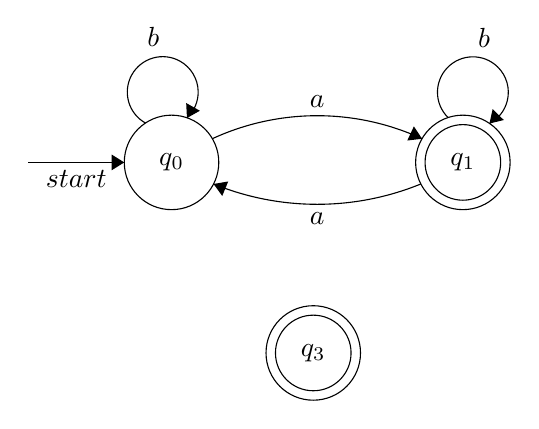
\begin{tikzpicture}[scale=0.2]
        \tikzstyle{every node}+=[inner sep=0pt]
        \draw [black] (16.1,-27) circle (3);
        \draw (16.1,-27) node {$q_0$};
        \draw [black] (34.6,-27) circle (3);
        \draw (34.6,-27) node {$q_1$};
        \draw [black] (34.6,-27) circle (2.4);
        \draw [black] (25.1,-39.1) circle (3);
        \draw (25.1,-39.1) node {$q_3$};
        \draw [black] (25.1,-39.1) circle (2.4);
        \draw [black] (7,-27) -- (13.1,-27);
        \fill [black] (13.1,-27) -- (12.3,-26.5) -- (12.3,-27.5);
        \draw (10.05,-27.5) node [below] {$start$};
        \draw [black] (18.69,-25.495) arc (114.75276:65.24724:15.906);
        \fill [black] (32.01,-25.5) -- (31.49,-24.71) -- (31.07,-25.61);
        \draw (25.35,-23.53) node [above] {$a$};
        \draw [black] (31.934,-28.368) arc (-67.77817:-112.22183:17.409);
        \fill [black] (18.77,-28.37) -- (19.32,-29.13) -- (19.7,-28.21);
        \draw (25.35,-30.16) node [below] {$a$};
        \draw [black] (14.455,-24.505) arc (241.12502:-46.87498:2.25);
        \draw (14.95,-19.7) node [above] {$b$};
        \fill [black] (17.08,-24.18) -- (17.9,-23.72) -- (17.03,-23.23);
        \draw [black] (33.67,-24.16) arc (225.8699:-62.1301:2.25);
        \draw (35.95,-19.71) node [above] {$b$};
        \fill [black] (36.29,-24.53) -- (37.2,-24.31) -- (36.49,-23.61);
    \end{tikzpicture}
\end{center}

Автоматы удобно представлять не набором множеств, а автоматом (Диаграмма Мура).

Каждое состояние обозначаем отдельным кругом (внутри впишем название состояния). Двойной кружок - принимающее состояние. Входная стрелка у начального состояние. Определим переходы: переход из состояния из $q_0$ в $q_1$ по символу a обозначим стрелкой. Впишем обратный переход. Петля будет вести из данного состояния в него же.

Автомат принимает слово с точки зрения графов - есть путь из начального состояния в принимающее, если автомат ДКА, то это путь определенном однозначно, для НКА не обязательно путь должен быть определен однозначно, и вдоль этого пути написано наше слово, принадлежность которого мы проверяем.

Распишем формально наш автомат.
\begin{enumerate}
    \item {\bfseries\itshape{Q}} - \{$q_0, q_1, q_3$\}
    \item $\boldsymbol{\Sigma}$ - \{$a,b$\};
    \item $\boldsymbol{q_0}$ -$q_0$
    \item $\boldsymbol{\delta}$ : $(\{q_0,b,q_0\}, \{q_0,a,q_1\},\{q_1,b,q_1\},\{q_1,a,q_0\})$
    \item $\boldsymbol{F} \subset \boldsymbol{Q}$ - \{$q_1,q_3$\}
\end{enumerate}

\textbf{Конфигурация автомата}
Конфигурацией конечного автомата называется $\mathcal{A} = \langle Q, \Sigma, q_s, F, \delta\rangle$ называется элемент множества $Conf(\mathcal{A}) = Q\times \Sigma^*$

\textbf{Отношение достижимости}
Зададим следующее отношение $\vdash^* \ \subset \ Conf(\mathcal{A})^2$:
\begin{itemize}
    \item $\forall q \in Q, w \in \Sigma^*: (q, w) \vdash^* (q, w)$
    \item $(q_1, xay) \vdash^* (q_2, ay) \vee (q_2, a, q_3) \in \delta \Rightarrow (q_1, xay) \vdash^* (q_3, y).$
\end{itemize}
Если $\forall x: (p, wx) \vdash^* (q, x)$, то будем писать $p \xrightarrow{w} q$.


\textbf{Слово принимаемое автоматом}
Будем говорить что слово $w$ принимается автоматом если для некоторого $q_f \in F$ верно $(q_s, w) \vdash^* (q_f, \varepsilon)$. Иначе говоря, если <<идя по стрелочкам>> в автомате по этому слову и правильно выбирая путь можно дойти до финального состояния.

\textbf{Язык принимаемый автоматом}
Язык автомата $\mathcal{A}$ --- это множество $L(\mathcal{A})$ всех слов принимаемых автоматом. Будем говорить, что конечный автомат принимает язык $B$ если $B = L(\mathcal{
        A})$. Будем говорить что два автомата $\mathcal{A}, \mathcal{B}$ эквивалентны, если $L(\mathcal{A})=L(\mathcal{B})$.

\textbf{Автоматный язык}
Язык называется автоматным если он принимается каким-либо конечным автоматом.

\textbf{Теорема Клини}
Класс автоматных языков и класс регулярных языков совпадают.

\begin{definition}{}{}
    $FollowPos(i \sigma)$ - {i $\sigma'$: i $\sigma'$ может идти в слове после $i\sigma$}
\end{definition}


Будем строить ДКА по следующему РВ с помощью вспомогательного множества --- $FollowPos$
\[
    R = \underset{0}{\rhd}(\underset{1}{a}\underset{2}{a}|\underset{3}{b})^{*}\underset{4}{b}(\underset{5}{a}|\underset{6}{b})^{*}\underset{7}{a}\underset{8}{\lhd}.
\]

Чтобы вычислить множество $FollowPos$, нам понадобится представление формулы в виде графа, который называется синтаксическим деревом:


\begin{figure}[h!tp]
    \centering
    \includegraphics[scale=0.5]{images/SintTree.PNG}
    \caption{Синтаксическое дерево}
    \label{fig:SyntaxTree1}
\end{figure}

Как же с помощью него вычислять функцию $FollowPos$? На самом деле одного синтаксического дерева недостаточно, нам придется ввести ещё три специальных атрибута. Пусть $u$ - узел синтаксического дерева, тогда:
\begin{definition}Символом $f_{u}$ будем обозначать значение атрибута $FirstPos(u)$ "--- множество номеров позиций, с которых может начинаться слово из $R_u$, где ($R_u$ - регулярное выражение, задаваемое вершиной $u$) \end{definition}

\begin{definition}
    Символом $l_{u}$ будем обозначать значение атрибута $LastPos(u)$ "--- множество номеров позиций, в которых может заканчиваться слово из $R_u$, где ($R_u$ - регулярное выражение, задаваемое вершиной $u$)
\end{definition}

\begin{definition}
    Атрибут $nullable(u)$ показывает содержит ли $R_u$ пустое слово ($T$ и $F$)
\end{definition}

Эти атрибуты вычисляются снизу вверх: зная атрибуты дочерних
узлов, вычисляются атрибуты родителя.
\begin{figure}[h!tp]
    \centering
    \includegraphics[scale=0.5]{images/7.PNG}
    \caption{Вычисление атрибутов для одного из узлов}
    \label{fig:SampleNode}
\end{figure}

В примере на рисунке $2$ левый узел имеет атрибут $nullable$ равный $True$, а значит конкатенация (корень данного поддерева) может начинаться как с $f_u$, так и с $f_v$. С другой стороны итоговая конкатенация может заканчиваться только с $f_v$, так как правый узел имеет атрибут $nullable$ равный $False$. Атрибут $nullable$ итоговой конкатенации тоже будет равен $False$, так как мы конкатенируем слова, одно из которых точно не может оказаться пустым.


После нескольких итераций вычислений таких атрибутов мы получаем готовое синтаксическое дерево:
\begin{figure}[h!t!p]
    \centering
    \includegraphics[scale=0.5]{images/FullSintTree.PNG}
    \caption{Готовое синтаксическое дерево}
    \label{fig:SyntaxTree2}
\end{figure}


Теперь, используя рисунок, мы можем найти необходимое множество $FollowPos$ по следующему алгоритму:
\begin{enumerate}
    \item Положим сначала $FollowPos(i) = \varnothing$ для каждого номера $i$
    \item Для каждой вершины-конкатенации $u\cdot v$, для каждого $i \in LastPos(u)$ добавим к $FollowPos(i)$ множество $FirstPos(v)$.
    \item Для каждой вершины-итерации $u^{*}$, для каждого $i \in LastPos(u)$ добавим к
          \\$FollowPos(i)$  множество $FirstPos(u)$.
\end{enumerate}

Построим таблицу множества $FirstPos$ для нашего регулярного выражения:
\begin{table}[h!]
    \centering
    \begin{tabular}{c|c}
        $i$   & $FollowPos(i)$ \\ \hline
        $1_a$ & $2_a$          \\
        $2_a$ & $1_a,3_b,4_b$  \\
        $3_b$ & $1_a,3_b,4_b$  \\
        $4_b$ & $5_a,6_b,7_a$  \\
        $5_a$ & $5_a,6_b,7_a$  \\
        $6_b$ & $5_a,6_b,7_a$  \\
        $7_a$ & $8_{\lhd}$
    \end{tabular}
    \caption{множество $FirstPos$}
\end{table}

Теперь с помощью таблицы с $FirsPos$ мы можем построить следующий ДКА:
\begin{figure}[ht!p]
    \centering
    \includegraphics[scale=0.5]{images/DKA.PNG}
    \caption{ДКА по таблице $FirstPos$}
    \label{fig:DFA}
\end{figure}

Начальное состояние автомата "--- это корень синтаксического дерева, поскольку атрибут $FirstPos(\text{Корень})$ как раз и будет указывать нам $FollowPos$ в самом начале. Далее проходим по таблице и строим итоговый автомат.


$\delta(S,b) = \bigcup followpos(\bigcup b)$

Проблема данного алгоритма в том, что если вы возьмете РВ и построите по нему ДКА, то оно окажется очень большим. Из-за экспоненциального роста возникают проблемы с памятью. Чтобы решить данную проблему зачастую используют НКА.

Алгоритм построения НКА мы рассмотрим на следующей лекции, а сейчас давайте построим НКА использую такой же  формализм, что и выше.

Начальное состояние - нулевая позиция. Из него будеь переход по $\varepsilon$ во все позиции, с которых слово может начинается.

Дальше для каждого отдельного символа и для каждой отдельной позиции будет просто переходы во все позиции по $followpos$. Мы уже знаем, что по символу $a$ идет переход в позицию $2a$. Из кружка, в котором написан символ позиции, идет переход во все кружки с $followpos$ от этой позиции и на переходе будет написан этот символ. Но всюду придется заменить маркер начала слова на пустое слово, и в конце добавляем новую вершину - маркер конца слова, и это состояние сделаем принимающим.

Еще раз алгоритм построения:
\begin{enumerate}
    \item Множество состояний это множество позиций
    \item Из позиции есть переход во все позиции из множества $followpos$ этот переход должен быть именно по символу из $followpos$
    \item Принимающее состояние единственное - маркер конца слова
    \item Все выходы из принимающего состояния - эпсилон переходы
\end{enumerate}


\begin{center}
    \begin{tikzpicture}[scale=0.2]
        \tikzstyle{every node}+=[inner sep=0pt]
        \draw [black] (21.1,-22.9) circle (3);
        \draw (21.1,-22.9) node {$\rhd$};
        \draw [black] (40.6,-14.5) circle (3);
        \draw (40.6,-14.5) node {$1_a$};
        \draw [black] (41.9,-26.2) circle (3);
        \draw (41.9,-26.2) node {$3_b$};
        \draw [black] (27.9,-35.9) circle (3);
        \draw (27.9,-35.9) node {$4_b$};
        \draw [black] (53.2,-14.5) circle (3);
        \draw (53.2,-14.5) node {$2_a$};
        \draw [black] (41.2,-36.6) circle (3);
        \draw (41.2,-36.6) node {$\lhd$};
        \draw [black] (41.2,-36.6) circle (2.4);

        \draw [black] (43.6,-14.5) -- (50.2,-14.5);
        \fill [black] (50.2,-14.5) -- (49.4,-14) -- (49.4,-15);
        \draw (46.9,-15) node [below] {$a$};
        \draw [black] (23.86,-21.71) -- (37.84,-15.69);
        \fill [black] (37.84,-15.69) -- (36.91,-15.54) -- (37.31,-16.46);
        \draw (31.84,-19.21) node [below] {$\varepsilon$};
        \draw [black] (24.06,-23.37) -- (38.94,-25.73);
        \fill [black] (38.94,-25.73) -- (38.23,-25.11) -- (38.07,-26.1);
        \draw (31.09,-25.15) node [below] {$\varepsilon$};
        \draw [black] (22.49,-25.56) -- (26.51,-33.24);
        \fill [black] (26.51,-33.24) -- (26.58,-32.3) -- (25.7,-32.76);
        \draw (23.82,-30.55) node [left] {$\varepsilon$};
        \draw [black] (30.9,-36.06) -- (38.2,-36.44);
        \fill [black] (38.2,-36.44) -- (37.43,-35.9) -- (37.38,-36.9);
        \draw (34.49,-36.81) node [below] {$b$};
        \draw [black] (9.9,-22.9) -- (18.1,-22.9);
        \fill [black] (18.1,-22.9) -- (17.3,-22.4) -- (17.3,-23.4);
        \draw (14,-23.4) node [below] {$start$};
    \end{tikzpicture}
\end{center}

Очевидно, регулярность будет сохраняться для любых композиций приведенных выше операций. Поэтому регулярным языком будет результат любой операции, которую можно, так сказать, "выразить в элементарных функциях". \\
Например, симметрическая разность двух регулярных языков:
\[X \triangle Y = (X \ \backslash \ Y) \cup (Y \ \backslash \ X) = (X \cup Y) \ \backslash \ (Y \cap X)\]
будет регулярным языком. \\
Разность двух регулярных языков также будет регулярна, так как
\[X \ \backslash \ Y = X \cap \overline{Y}\]

    \section{Контекстно-свободные грамматики. Автоматы с магазинной памятью. Эквивалентность
    автоматов с магазинной памятью и контекстно-свободных грамматик.}

    \section{Архитектура Фон-Неймана. Принципы однородности памяти, адресности и
    программного управления. Гарвардская архитектура, отличия от архитектуры Фон-
    Неймана. Примеры реализаций.}

    \section{Абстрактные структуры данных: списка, вектора, деревья поиска. Их асимптотики для
    операций поиска элемента и вставки новых элементов в середину или конец. Примеры
    реализаций.}

    \section{Целочисленная арифметика в представлении компьютера. Знаковые и беззнаковые
    значения, способы представления отрицательных значений. Целочисленное
    переполнение и его контроль. Длинная целочисленная арифметика.}
    \columnbreak

    \section{Вещественная арифметика. Представления с фиксированной и плавающей точкой.
    Стандарт IEEE754. Специальные вещественные значения, определенные стандартом
    IEEE754 и операции над ними.}

    \section{Устройство виртуального адресного пространства процесса. Стек и куча. Динамическая
    загрузка библиотек. Механизм трансляции адресов из виртуального в физическое
    адресное пространство.}
    \section{Операционные системы и их компоненты. Ядро операционных систем. Системные
    вызовы и их отличия от обычных библиотечных функций. Способы реализации
    системных вызовов (прерывания, sysenter, syscall).}
    \subsection*{Компоненты операционной системы}

      \begin{definition}{}{}
        \textit{Ядро} --- программа, которая запускается самой первой. Имеет привилегированное положение на процессоре и может взаимодействовать с <<железом>> напрямую.
      \end{definition}

      \begin{definition}{}{}
        \textit{Базовые библиотеки}: зачастую входят в состав операционной системы, потому что привязаны к определенному ядру (версии ядра), чтобы максимально использовать его функциональность. 
      \end{definition}

      \begin{definition}{}{}
      \textit{Служебные сервисы} --- ведение логов, обработка сетевых соединения, и т.д.
      \end{definition}

      \begin{definition}{}{}
      \textit{Минимальная пользовательская оболочка} --- чтобы пользователь мог взаимодействовать с системой.
      \end{definition}

      \subsection*{Процессы}

      \begin{definition}{}{}
      \textit{Процесс} --- любой экземпляр программы, работающей в операционной системе.
      \end{definition}

      Примеры:
      \begin{itemize}
        \item Приложения
        \item Фоновые сервисы (демоны)
        \item Команды в терминале
      \end{itemize}

      Главные команды для мониторинга процессов:
      \begin{itemize}
        \item ps -A -- список процессов
        \item pstree -- иерархия процессов
        \item top
      \end{itemize}

      \subsection*{UNIX программы}

      Программы:
      \begin{itemize}
        \item \textbf{Бинарные исполняемые файлы.}
        \item \textbf{Текстовый файл, начинающийся с \#!.} После \#! указывается путь к интерпретатору (например, \#!/bin/bash). Это могут быть скрипты на Python/Perl/Escript или Shell скрипт.
      \end{itemize}

      Название файла и его расширение не имеет значения. Любой файл, имеющий атрибут 
      <<исполняемый>> является программой.

      \subsection*{UNIX пользователи}

      Единственные привилегированный пользователь: root (UID = 0).

      Непривилегерованные пользователи:
      \begin{itemize}
        \item Реальные пользователи, которые могут войти в систему (UID $\ge$ 1000)
        \item Фейковые пользователи, привязанные к сервисам (UID $<$ 1000).
      \end{itemize}

      \textbf{Зачем сервисам нужны фейковые пользователи?}
      Допустим, у вас есть веб-сервер и сервер баз данных. Теоретически какой-то пользователь
      может подключиться к веб-серверу и найти там уязвимость. Для того, чтобы 
      минимизировать возможный ущерб от уязвимости в одном из процессов, процессы запускаются
      под разными пользователями и не имеют права общаться друг с другом.

      Непривилегерованные пользователи могут временно получить 
      дополнительные привилегии:

      \begin{itemize}
        \item su - запускает терминал от имени root
        \item sudo - запускает любую программу от имени root
        \item Запустить программу с атрибутом SUID и владельцем root. SUID атрибут означает, что при запуске программа
        исполняется от того пользователя, кто является владельцем файла. Кстати, так и 
        работает команда sudo, владелец sudo - root, а также у sudo проставлен атрибут SUID.
        \item Запустить программу с <<capabilities>> флагами. Эти флаги позволяют тонко настроить, что можно делать программе, а что - нельзя.
      \end{itemize}

      \subsection*{UNIX межпроцессорное взаимодействие}

      Процессы работают изолированно друг от друга. Единственный способ взаимодействовать друг с другом --- использовать методы межпроцессорного взаимодействия ядра (Inter-Process Communication, IPC):

      \begin{itemize}
        \item {Сигналы} для коротких сообщений
        \item {Каналы и сокеты} для последовательных данных
        \item {Разделяемая память}, в которой хранятся большие куски данных
      \end{itemize}

      \subsection*{Процесс запуска}

      \begin{enumerate}
        \item {Загрузчик} с диска или UEFI материнской платы выполняется в привилегированном режиме
        \item Загрузчик запускает {ядро}, тоже в привилегированном режиме.
        \item Ядро запускает первый непривелигерованный процесс: {init или systemd}.
      \end{enumerate}

      \subsection*{Сервисы (``Демоны'')}
      \begin{definition}{}{}
        \textit{Сервисы} --- это специальные системные службы, которые работают в фоновом режиме.
      \end{definition}

      Минимальный сет во многих системах:

      \begin{itemize}
        \item \textbf{dhclient} -- держит активным полученный IP адрес в сети
        \item \textbf{getty} -- переключение между графическим/консольным входом в систему
        \item \textbf{sshd} -- подключение по ssh
        \item \textbf{ntpd или chronyd} -- синхронизация времени
        \item \textbf{syslogd} -- системный лог
      \end{itemize}

      \subsection*{\#!/bin/sh}

      В терминале вы работаете в интерпретаторе \texttt{shell}. \texttt{shell} предоставляет возможность выполнять
      команды и последовательности команд.

      Бывают разные интерпретаторы \texttt{shell}:
      \begin{itemize}
        \item самодостаточный \texttt{shell} program: \textbf{FreeBSD}
        \item основной в \texttt{Linux}: \textbf{bash}
        \item debian: \textbf{dash}
        \item alpine: \textbf{busybox}
        \item maxOS X: \textbf{zsh}
      \end{itemize}

      \subsection*{Системный демон (systemd)}
      \begin{definition}{}{}
      Процесс, который управляет всеми остальными процессами. При этом сам является обычным процессом. \texttt{Systemd} пришел на замену INIT-процессу.

      \end{definition}

      Чем systemd лучше?
      \begin{itemize}
        \item Устранение интерпретации \texttt{shell} скриптов. 
        \item Запуск сервисов параллельно
      \end{itemize}

      \subsubsection*{Концепты systemd}

      \begin{itemize}
        \item Сервисы
        \item Цели:
          \begin{itemize}
            \item \textit{Стандартные цели}. Например, уровни \texttt{init} в System-V:
              \begin{itemize}
                \item poweroff.target (init 0)
                \item rescue.target (init 1)
                \item multi-user.target (init 3)
                \item graphical.target (init 5)
                \item reboot.target (init 6)
                \item sleep.target и hibertate.target (не присутствуют в System-V)
              \end{itemize}
            \item \textit{Специальные цели}
          \end{itemize}
      \end{itemize}

      \subsection*{Фоновые задачи}

      \begin{itemize}
        \item \textbf{Нет привязанного к задаче терминала.} Для того, чтобы сигнал \texttt{SIGHUP}
        не останавливал исполнение задачи используется команда \texttt{nohup}.
        \item \textbf{Пишут в лог.} Иногда пишут данные в какую-то старинную 
        локальную почтовую систему.
        \item \textbf{Запускается в единственном экземпляре.} Обычно это достигается
        с помощью file lock.
      \end{itemize}

      \subsection*{Дистрибутивы \texttt{Linux}}

      Ядро называется Linux. Базовая система --- минимальная юзабельная система.

      \textit{Дистрибутив}:
      \begin{itemize}
        \item Ядро
        \item Базовая система
        \item GUI оболочка
        \item Программное обеспечение 
      \end{itemize}

      \subsubsection*{Какие есть дистрибутивы?} 

      Общего назначения:
      \begin{itemize}
        \item OpenSUSE
        \item Fedora
        \item Debian
        \item Ubuntu
      \end{itemize}

      Специфические дистрибутивы:
      \begin{itemize}
        \item Alpine Linux --- очень легковесный, поэтому его
        хорошо ставить на виртуальную машину.
        \item Kali Linux --- используется для тестов на безопасность.
      \end{itemize}
      \begin{definition}{}{}
        \underline{Прерывание} --- это сигнал от программного или аппаратного обеспечения,
        сообщающий процессору о наступлении какого-либо события, требующего немедленного внимания.
      \end{definition}
      
      \subsection*{Обработка прерывания в x86}
      
      \begin{itemize}
        \item Каждое устройство имеет свой собственный номер прерывания (IRQ).
        \item Процессор получает сигнал INT и прекращает исполнение текущекого контекста.
        \item Каждое прерывание имеет свой адрес в векторе прерываний.
        \item Прерывания бывают не только аппаратные. Его можно сымитировать, 
        вызвав прерывание программно.
      \end{itemize}
      
      \subsection*{Маска прерывания}
      
      Иногда хочется запретить прерывания в каком-то месте. Для этого существует маска прерываний.
      
      \subsection*{Номера прерываний}
      
      \begin{itemize}
        \item 0 --- нажатие на кнопку включения или Reset
        \item 1...15 --- Аппаратные прерывания. Тут задействованы реальные железяки.
        \item 16+ --- программные прерывания, вызванные через int.
      \end{itemize}
      
      \subsection*{Базовый вектор прерываний}
      
      Кто прописывает нам функции, которые будут вызваны при прерывании?
      \begin{itemize}
        \item BIOS --- содержит весь минимальный набор функций, нужный после включения.
        \item Обработка железяк (клавиатура, ...).
        \item Функции для обращения к данным на диске и загрузки операционной системы.
      \end{itemize}
      
      \subsection*{Обработка прерываний}
      
      \begin{itemize}
        \item Сохранить EIF на стек
        \item Проставить 1 в флаг IF
        \item Перейти на инструкцию по адресу IDTR + offset
      \end{itemize}
      
      \underline{Перед вызовом обработчика прерывания:}
      \begin{itemize}
        \item Сбросить флаги
        \item Переключить текущее адресное пространство
        \item Заменяется стек
      \end{itemize}
      
      \underline{Выполнение функции обработчика прерывания:}
      \begin{itemize}
        \item Сохранить текущее значение регистров и флагов
        \item что-то поделать...
        \item бернуть состояние регистров и флагов обратно
      \end{itemize}
      
      \subsection*{Ядро}
      
      При запуске операционной системы есть одна программа - ядро. Она может делать все что угодно.
      
      \subsection*{Режимы исполнения (x86)}
      
      \textbf{Обычный режим:}
      \begin{itemize}
        \item Процесс имеет доступ только к своей собственной памяти.
        \item Виртуальное адресное пространство каждого процесса начинается с адреса 0.
        \item Процесс не может взаимодействовать с устройствами.
      \end{itemize}
      
      \textbf{Превилегированный режим:}
      \begin{itemize}
        \item Полный доступ к физической (не виртуальной) памяти.
        \item Полный доступ к портам ввода/вывода.
        \item Некоторые дополнительные команды, не доступные в обычном режиме исполнения.
      \end{itemize}
      
      \begin{definition}{}{}
        \underline{Системный вызов} --- механизм для взаимодействия обычных процессов с ядром. 
        Он позволяет обратиться к функциональности ядра, чтобы сделать недоступные в обычном
        режиме операции.
      \end{definition}
      
      \subsection*{Ядро}
      
      \begin{itemize}
        \item Обычный ELF файл.
        \item Запускается в привилегированном режиме.
        \item Отвечает за взаимодействие с железом.
      \end{itemize}
      
      \subsection*{Запуск ядра}
      
      \begin{itemize}
        \item Проинициализировать устройства.
        \item Проинициализировать вектор прерываний.
        \item Найти, загрузить и запустить все драйвера.
        \item Понизить привилегии процессора.
        \item Запустить первый пользовательский процесс --- init.
      \end{itemize}
      
      \subsection*{Взаимодействие с ядром (x86)}
      
      \begin{itemize}
        \item Все процессы непривилегированы.
        \item Единственный способ получить доступ к железу --- переключиться в 
        режим ядра.
        \item Все прерывания переключают процессор в привилегированный режим.
        \item Используйте int для того, чтобы получить доступ к системным вызовам.
      \end{itemize}
      
      \subsection*{Типы архитектуры ядер}
      
      \begin{itemize}
        \item \textbf{Монолитные ядра.} Одна большая программа, которая исполняется 
        в привилегированном режиме. Примеры: Linux.
        \item \textbf{Микроядерная.} Только небольшая часть ядра запускается в привилегированном
        режиме. Большая часть подсистем работает как пользовательские процессы. Примеры: Minix3.
        \item \textbf{Гибридная.} Модульная, но не одна большая программа, запускаемая в
        привилегированном режиме. Примеры: Windows, Mac, BSD или Linux.
      \end{itemize}
      
      \subsection*{Системные вызовы}
      
      Системный вызов можно осуществить с помощью:
      \begin{itemize}
        \item int 0x80 (Linux, BSD)
        \item sysenter/sysleave инструкции (Intel)
        \item syscall/sysret инструкции (AMD64/x86\_64)
      \end{itemize}
      
      \subsection*{INT 0x80}
      
      \begin{itemize}
        \item В eax сохраняется номер системного вызова
        \item Параметры сохраняются в ebx, ecx, ...
        \item Возвращаемое значение сохраняется в eax
        \item Конвенции вызовов отличаются от принятых в языке C!
      \end{itemize}
      
    \section{Процессы и потоки. Сходства и различия между ними. Реализация многозадачности и
    алгоритмы планирование задач в операционных системах.}
    \subsection*{Что такое процесс?}

    \begin{definition}{}{}
      \underline{Процесс} --- это экземпляр программы в одном из состояний выполнения. Каждый
      из процессов выполняется в своем изолированном адресном пространстве.
    \end{definition}
    
    \subsection*{Аттрибуты процесса}
    
    Память:
    \begin{itemize}
      \item Значения регистров процессора.
      \item Таблицы и каталоги страниц виртуального адресного пространства.
      \item Private и Shared страницы памяти.
      \item Отображение файлов в память.
      \item Отдельный стек в ядре для обработки системных вызовов.
    \end{itemize}
    
    Файловая система:
    \begin{itemize}
      \item Таблица файловых дескрипторов.
      \item Текущий каталог.
      \item Корневой каталог.
      \item Маска аттрибутов создания нового файла umask. 
    \end{itemize}
    
    Другие аттрибуты:
    \begin{itemize}
      \item Переменные окружения
      \item Лимиты
      \item Счетчики ресурсов
      \item Идентификаторы пользователя и группы
    \end{itemize}
    
    \subsection*{Информация о процессах}
    
    Команда \textbf{ps} показывает список процессов, \textbf{top} --- потребление ресурсов.
    
    \subsection*{Жизненный цикл процессов}
    
    \begin{itemize}
      \item Выполняется (Running)
      \item Остановлен (Stopped)
      \item Временно приостановлен
        \begin{itemize}
          \item Suspended --- может быть завершен
          \item Disk Suspended --- не может быть завершен
        \end{itemize}
      \item Исследуется (Tracing)
      \item Зомби (Zombie)
    \end{itemize}
    
    \textbf{Как устроен планировщик заданий?}
    
    \subsection*{Round Robin}
    \textit{Windows 9x, старые UNIX}
    
    Аппаратный таймер время от времени генерирует прерывание, после чего планировщик
    выбирает, какой процесс будет выполняться дальше.
    
    \subsection*{Приоритет}
    
    \begin{definition}{}{}
      \underline{Приоритет процесс} --- это численное значение от -20 до 19. 
      Оно обозначает то, сколько раз пропустить планировщиком заданий.
    \end{definition}
    
    \begin{itemize}
      \item Значение от 
      \item Численное значение --- 
    \end{itemize}
    
    \subsection*{Многоуровневая очередь}
    \textit{Linux, xBSD, Mac, Windows}
    
    Эта схема отталкивается от того, что есть два типа процессов:
    \begin{itemize}
      \item Не очень активно взаимодействующие с внешним миром (что-то вычисляют). 
      Им надо просто не мешать выполняться. 
      \item Много взаимодействующие с пользователем. Их надо переключать быстро.
    \end{itemize}
    
    Есть набор очередей, уровней, которые рассположены по увеличению времени переключения.
    При переключении очереди, если процесс освободил процессор до следующего события, он
    перемещается в следующую очередь (более редко переключаемую), иначе --- в предыдущую.
    
    \subsection*{Ничегонеделание}
    
    while (1) {
      // Так делать очень плохо, потому что вы загружаете процессор
    }
    
    while (1) {
      sched\_yield(); // Передаем управление другому процессу
    }
    
    \subsection*{Создание процесса}
    
    Системный вызов fork().

    \subsection*{Копия процесса}
    
    При fork создается полная копия процесса. Память, регистры, ... --- точная копия.
    
    Не копируются:
    \begin{itemize}
      \item eax, rax
      \item Сигналы, ожидающие доставки
      \item Таймеры
      \item Блокировки файлов
    \end{itemize}
    
    \textbf{В связи с копированием всего адресного пространства может возникать необычное поведение.} Например, 
    буфер ввода и вывода тоже копируется. Поэтому если не сделать fflush, один и тот
    же текст может продублироваться.
    
    \subsection*{Ограничения}
    
    /proc/sys/kernel/pid\_max --- максимальное число одновременно запущенных процессов.
    /proc/sys/kernel/threads\_max --- максимальное число одновременно 
    выполняющихся потоков (каждый процесс --- уже один поток).
    
    \subsection*{Дерево процессов}
    
    \begin{itemize}
      \item Процесс с номером 1 --- systemd
      \item У каждого процесса кроме systemd есть свой родитель
      \item Если родитель процесса умирает, то его родителем становится systemd.
      \item Если ребенок умирает, про это узнает его родитель. 
    \end{itemize}
    
    \subsection*{Завершение работы процесса}
    
    \begin{itemize}
      \item Системный вызов \_exit(int)
      \item Функция exit(int)
      \item Оператор return в main
    \end{itemize}
    
    \subsection*{Ожидание завершения процесса}
    
    Системный вызов waitpid.
    
    \subsection*{Zombie процессы}
    
    Удалением зомби из таблицы процессов занимается родитель --- 
    вызовом wait или waitpid.
    
    \subsection*{exec}
    
    Системный вызом exec позволяет заместить тело процесса другой программой.
    
    \subsection*{Аттрибуты процесса, сохраняемые exec}
    
    \begin{itemize}
      \item Открытые файловые дескрипторы 
      \item Текущий каталог
      \item Лимиты процесса
      \item UID, GID
      \item Корневой каталог --- root.
    \end{itemize}
    \section{Проблема многопоточной синхронизации. Атомарные переменные и объекты
    блокировки. Неблокирующие структуры данных и их реализация.}
    \section{Интерконнект в вычислительном кластере. Отличие интерконнекта от глобальных
    компьютерных сетей. Основные характеристики интерконнекта. Топологии соединений
    узлов в вычислительном кластере, характеристики топологий.}
    \columnbreak

    \section{Понятие ускорения и масштабируемости параллельных программ. Закон Амдала.
    Оценка эффективности параллельных программ. Ярусно-параллельная форма
    программы.}

    \section{Параллельные и распределённые вычислительные системы. Парадигма Map-Reduce.
    Примеры, отличия. Распределенные файловые системы. Особенности хранения файлов
    в них. Репликация.
    }
\end{multicols}